\documentclass[11pt,letterpaper]{article}
\PassOptionsToPackage{hyphens}{url}
\usepackage[margin=.83in,top=.8in,bottom=.8in,headheight=15pt]{geometry}
\usepackage[T1]{fontenc}
\usepackage{lmodern,amsmath,amssymb,mathtools,bm,booktabs,array,graphicx,tikz}
\usetikzlibrary{arrows.meta,positioning,calc,decorations.pathreplacing,patterns}
\definecolor{ink}{HTML}{17344D}\definecolor{accent}{HTML}{087E8B}\definecolor{pale}{HTML}{EDF5F5}\definecolor{gold}{HTML}{AD6B19}
\providecommand{\dd}{\,\mathrm{d}}\providecommand{\R}{\mathbb{R}}
\providecommand{\E}{\mathbb{E}}\providecommand{\Var}{\operatorname{Var}}
\providecommand{\Cov}{\operatorname{Cov}}\providecommand{\diag}{\operatorname{diag}}
\providecommand{\norm}[1]{\left\lVert#1\right\rVert}
\providecommand{\abs}[1]{\left|#1\right|}
\usepackage{microtype,hyperref,fancyhdr,enumitem,amsthm,sectsty,needspace}
\allsectionsfont{\raggedright}
\hypersetup{colorlinks=true,linkcolor=ink,urlcolor=accent,pdfauthor={Zan Ahmad},pdftitle={Membrane currents and Hodgkin--Huxley gate kinetics / Lecture notes}}
\setlength{\parindent}{0pt}\setlength{\parskip}{6pt}\linespread{1.07}
\setlist{itemsep=3pt,topsep=4pt,leftmargin=*}
\emergencystretch=2em\clubpenalty=10000\widowpenalty=10000
\pagestyle{fancy}\fancyhf{}\fancyhead[L]{\small Mathematical Modeling}\fancyhead[R]{\small Lecture 9}
\fancyfoot[L]{\footnotesize Zan Ahmad}\fancyfoot[R]{\footnotesize\thepage}\renewcommand{\headrulewidth}{.3pt}
\newtheorem{proposition}{Proposition}\newtheorem{theorem}{Theorem}\newtheorem{lemma}{Lemma}
\theoremstyle{definition}\newtheorem{definition}{Definition}\newtheorem{example}{Example}
\numberwithin{equation}{section}
\begin{document}
{\small\scshape Mathematical Modeling\hfill Lecture 9}\par\medskip
{\raggedright\hyphenpenalty=10000\exhyphenpenalty=10000\LARGE\bfseries\color{ink} Membrane currents and Hodgkin--Huxley gate kinetics\par}\medskip
{\small Lecture notes}\par\bigskip
A membrane equation combines charge conservation with voltage-dependent conductance laws. We derive the gate equations and clamp solutions, state the complete neuronal rate convention, and construct a gate-preserving numerical method whose accuracy is assessed separately from its admissibility.

\section{Membrane capacitance and the sign of current}
\hypertarget{note-membrane-capacitance-and-the-sign-of-current}{}\label{note:membrane-capacitance-and-the-sign-of-current}
{\small \href{slides.html\#frame=membrane-charge-balance\&step=1}{Slides for this section}}\par
Let $V=\phi_{\mathrm{in}}-\phi_{\mathrm{out}}$ be membrane voltage, measured in millivolts. Ionic current density is positive outward; applied current density $I_{\mathrm{app}}$ is positive inward. A specific membrane capacitance $C$ stores charge per area, so charge balance gives
\[
\boxed{C\dot V=I_{\mathrm{app}}-I_{\mathrm{ion}}.}
\]
We use $C=1\,\mu\mathrm F/\mathrm{cm}^2$, time in milliseconds, and currents in $\mu\mathrm A/\mathrm{cm}^2$. These units are consistent because $\mu\mathrm F\cdot\mathrm{mV}/\mathrm{ms}=\mu\mathrm A$. Current density and total current are distinct: a uniform density $I$ over membrane area $A_m$ gives total current $A_m I$.

The cell is space clamped in the mathematical sense that one voltage represents the whole patch. This removes axial spatial currents. A voltage clamp is a different intervention: it prescribes the voltage in time and supplies the current required to enforce it. In a current-driven experiment the voltage must instead be solved from charge balance.
\section{Conductance, reversal potential, and channel gates}
\hypertarget{note-conductance-reversal-potential-and-channel-gates}{}\label{note:conductance-reversal-potential-and-channel-gates}
{\small \href{slides.html\#frame=conductance-and-electrochemical-driving-difference\&step=1}{Slides for this section}}\par
The adopted neuronal model contains sodium, potassium, and leak currents:
\[
I_{\mathrm{ion}}=g_{\mathrm{Na}}(V-E_{\mathrm{Na}})
+g_{\mathrm K}(V-E_{\mathrm K})+g_{\mathrm L}(V-E_{\mathrm L}).
\]
The reversal potential is the voltage at which that current vanishes. A positive conductance does not determine current direction: the sign is the sign of $V-E_j$. Conductance density is measured in $\mathrm{mS}/\mathrm{cm}^2$, so conductance times millivolts gives $\mu\mathrm A/\mathrm{cm}^2$.

The three gate variables $m,h,n$ lie in $[0,1]$. Sodium activation is represented by $m$, sodium availability by $h$, and potassium activation by $n$. The conductances are
\[
g_{\mathrm{Na}}=120m^3h,\qquad g_{\mathrm K}=36n^4,\qquad g_{\mathrm L}=0.3.
\]
The powers express the model assumption that three identical activation gates and one availability gate must all permit sodium conduction, while four identical gates must permit potassium conduction. Multiplication of probabilities uses an independence assumption; it is not a literal structural proof about every ion channel.

The present voltage convention uses
\[
(E_{\mathrm{Na}},E_{\mathrm K},E_{\mathrm L})=(45,-82,-59)\,\mathrm{mV}.
\]
These parameters and the rates below follow the current neuronal propagation notes. A different voltage origin requires consistent changes to reversal potentials and rate formulas. The resulting waveform is not a cardiac-cell calibration.
\section{Gate kinetics and the voltage-clamp solution}
\hypertarget{note-gate-kinetics-and-the-voltage-clamp-solution}{}\label{note:gate-kinetics-and-the-voltage-clamp-solution}
{\small \href{slides.html\#frame=gate-opening-and-closing\&step=1}{Slides for this section}}\par
For any gate $s\in\{m,h,n\}$, opening and closing give
\[
\dot s=\alpha_s(V)(1-s)-\beta_s(V)s.
\]
Under a fixed voltage, the nonnegative rates are constant. Define
\[
s_\infty(V)=\frac{\alpha_s}{\alpha_s+\beta_s},\qquad
\tau_s(V)=\frac1{\alpha_s+\beta_s}.
\]
Then $\dot s=(s_\infty-s)/\tau_s$, and integration gives
\[
s(t)=s_\infty+[s(0)-s_\infty]e^{-t/\tau_s}.
\]
The solution is a convex combination of the initial gate and its limiting value, so it remains in $[0,1]$. If both rates vanish, the gate stays at its initial value instead. For $\alpha=0.2$ and $\beta=0.8\,\mathrm{ms}^{-1}$, $s_\infty=0.2$ and $\tau=1\,\mathrm{ms}$. Starting from $0.9$ gives $s(3)=0.2+0.7e^{-3}\simeq0.23485$.

The companion clamp fixes $V=-20\,\mathrm{mV}$ and initializes gates from rest. Sodium activation rises rapidly, availability falls, and potassium activation rises more slowly. Their products yield a transient sodium conductance and a sustained potassium conductance. This experiment computes gate responses to a prescribed voltage, not a predicted voltage excursion.
\begin{center}\begin{minipage}{.98\linewidth}\centering
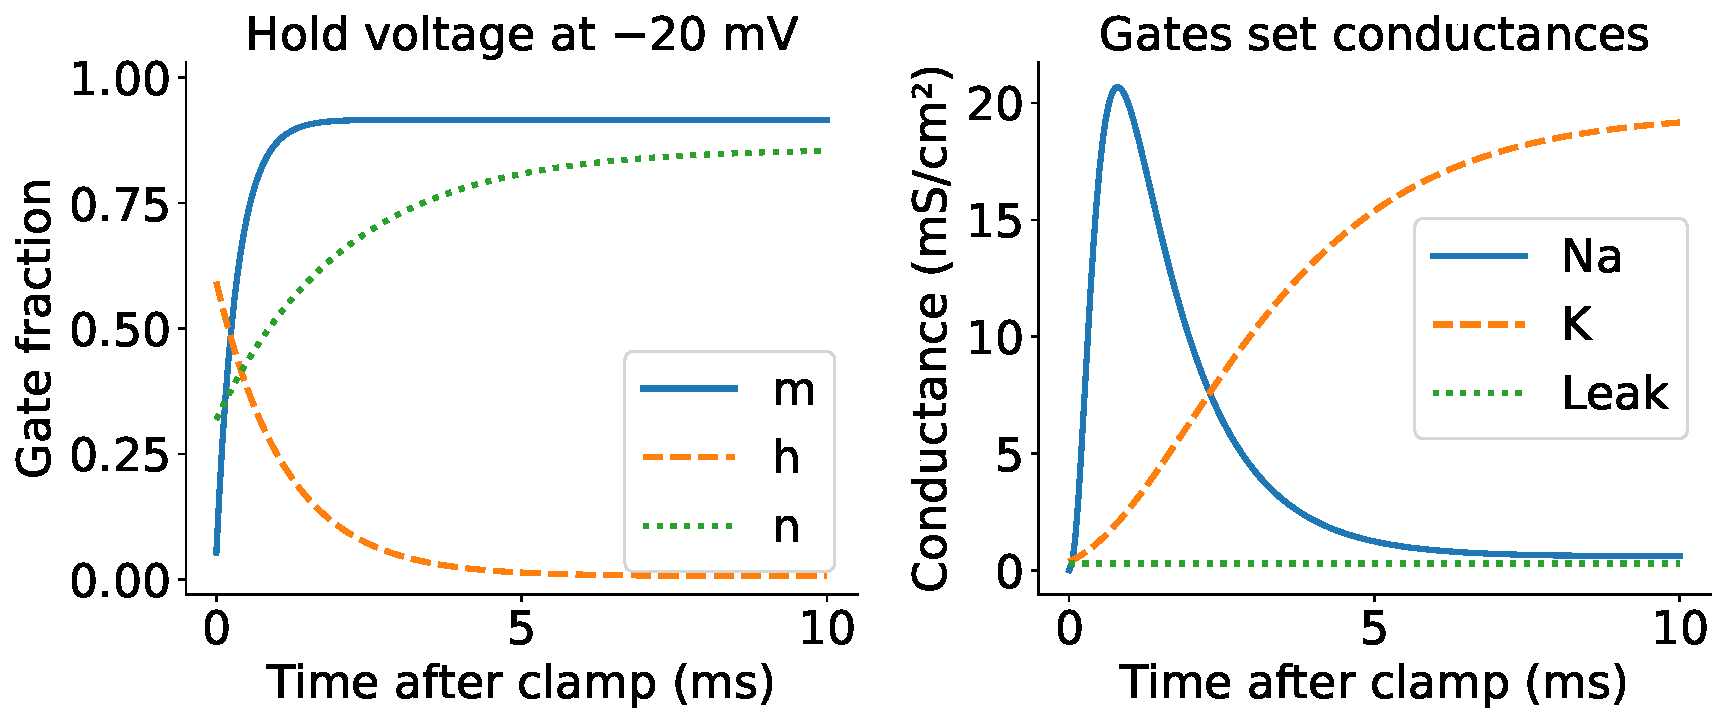
\includegraphics[width=.96\linewidth,height=.57\textheight,keepaspectratio]{voltage-clamp.pdf}\par\smallskip
{\small Synthetic voltage-clamp calculation at -20 mV, initialized from resting gates. Exact constant-rate gate solutions determine the sodium, potassium and leak conductances; voltage is prescribed rather than solved.}
\end{minipage}\end{center}
\section{Rate functions and removable singularities}
\hypertarget{note-rate-functions-and-removable-singularities}{}\label{note:rate-functions-and-removable-singularities}
{\small \href{slides.html\#frame=activation-rate-functions\&step=1}{Slides for this section}}\par
With $V$ numerically expressed in millivolts, define
\[
F(z)=\frac z{1-e^{-z}},\qquad F(0)=1.
\]
The gate rates, in $\mathrm{ms}^{-1}$, are
\[
\begin{aligned}
\alpha_m&=F((V+45)/10),&\beta_m&=4e^{-(V+70)/18},\\
\alpha_h&=0.07e^{-(V+70)/20},&\beta_h&=\frac1{1+e^{-(V+40)/10}},\\
\alpha_n&=0.1F((V+60)/10),&\beta_n&=0.125e^{-(V+70)/80}.
\end{aligned}
\]
Every exponent and argument is dimensionless; the constants in the voltage offsets and denominators carry the implicit millivolt unit. The apparent singularities at $V=-45$ and $V=-60\,\mathrm{mV}$ are removable. Taylor expansion gives
\[
F(z)=1+\frac z2+\frac{z^2}{12}-\frac{z^4}{720}+O(z^6).
\]
Direct evaluation of $1-e^{-z}$ loses accuracy near zero. The implementation uses this local series and otherwise computes the denominator as $-\operatorname{expm1}(-z)$. A division by zero or an arbitrary replacement by zero would change the kinetics at an ordinary voltage.
\section{Rest, feedback, and the pulse experiment}
\hypertarget{note-rest-feedback-and-the-pulse-experiment}{}\label{note:rest-feedback-and-the-pulse-experiment}
{\small \href{slides.html\#frame=a-self-consistent-resting-state\&step=1}{Slides for this section}}\par
At a zero-input equilibrium, each gate equals its voltage-dependent stationary value and ionic current balances:
\[
s=s_\infty(V_*),\qquad I_{\mathrm{ion}}(V_*,m_\infty,h_\infty,n_\infty)=0.
\]
The companion solves this scalar current equation for its adopted parameters and obtains $V_*\simeq-69.89767\,\mathrm{mV}$. It then computes the consistent gate values. A rounded voltage combined with inconsistent gates creates an artificial startup transient.

When voltage rises, sodium activation can increase inward sodium current, causing further depolarization. This positive feedback operates only over part of the trajectory. Falling sodium availability, increasing potassium conductance, and changing driving differences help terminate the excursion. Conductance and driving force must be interpreted together.

The synthetic experiment applies a rectangular inward current density from $1$ to $2\,\mathrm{ms}$. At $2\,\mu\mathrm A/\mathrm{cm}^2$ the response is small; at $10\,\mu\mathrm A/\mathrm{cm}^2$ it develops a spike that continues after the pulse ends. The notebook also examines $5\,\mu\mathrm A/\mathrm{cm}^2$. These cases do not locate a universal threshold: stimulus duration, initial state, and model parameters matter.
\begin{center}\begin{minipage}{.98\linewidth}\centering
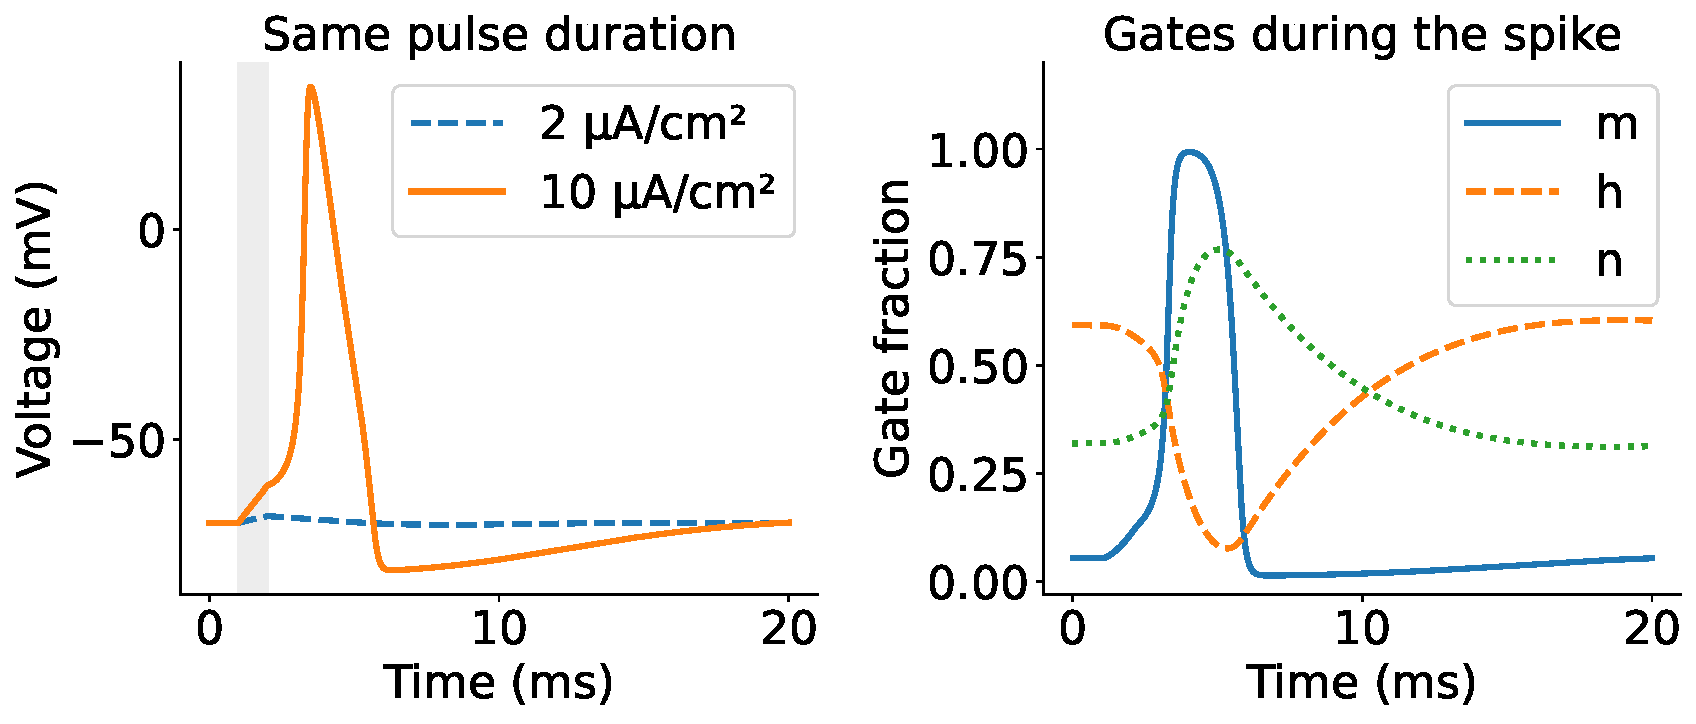
\includegraphics[width=.96\linewidth,height=.57\textheight,keepaspectratio]{pulse-and-gates.pdf}\par\smallskip
{\small Original single-compartment neuronal calculation, 0.005 ms nominal step. A rectangular inward current density is applied from 1 to 2 ms (gray band). The right panel shows m, h and n during the 10 $\mu$A/cm$^2$ experiment.}
\end{minipage}\end{center}
\section{A signed current calculation}
\hypertarget{note-a-signed-current-calculation}{}\label{note:a-signed-current-calculation}
{\small \href{slides.html\#frame=a-signed-ionic-current-sum\&step=1}{Slides for this section}}\par
For a hand calculation, prescribe $V=-60\,\mathrm{mV}$ and conductance densities
\[
(g_{\mathrm{Na}},g_{\mathrm K},g_{\mathrm L})=(0.12,0.36,0.30)\,\mathrm{mS}/\mathrm{cm}^2.
\] These are stated conductances, not values inferred from unspecified gate fractions. The outward-positive ionic currents are
\[
\begin{aligned}
I_{\mathrm{Na}}&=0.12(-60-45)=-12.6,\\
I_{\mathrm K}&=0.36(-60+82)=7.92,\\
I_{\mathrm L}&=0.30(-60+59)=-0.30,
\end{aligned}
\]
in $\mu\mathrm A/\mathrm{cm}^2$. Their sum is $-4.98$, an inward net ionic current. For inward applied current density $2$, the balance gives $\dot V=2-(-4.98)=6.98\,\mathrm{mV/ms}$. A $0.05$-millisecond Euler estimate therefore gives $V^+=-60+0.05(6.98)=-59.651\,\mathrm{mV}$. It is a local estimate, because voltage and conductances evolve over the interval.
\section{Gate-preserving integration of the coupled system}
\hypertarget{note-gate-preserving-integration-of-the-coupled-system}{}\label{note:gate-preserving-integration-of-the-coupled-system}
{\small \href{slides.html\#frame=an-exact-gate-substep\&step=1}{Slides for this section}}\par
The original teaching integrator uses two sequential substeps. For a time interval $\Delta t$, first freeze the voltage at $V^k$ and update each gate exactly:
\[
s^{k+1}=s_\infty(V^k)+[s^k-s_\infty(V^k)]e^{-\Delta t/\tau_s(V^k)}.
\]
Then compute the updated conductances, set $G=\sum_jg_j$ and
\[
V_{\mathrm{tar}}=\frac{I_{\mathrm{app}}+\sum_jg_jE_j}{G},
\]
and integrate the linear voltage equation with these conductances frozen:
\[
V^{k+1}=V_{\mathrm{tar}}+(V^k-V_{\mathrm{tar}})e^{-G\Delta t/C}.
\]
Leak conductance ensures $G>0$ here. Exact substeps do not make the coupled method exact. This sequential split has first-order consistency in the full state in general; a particular voltage-only experiment can show higher apparent convergence order.

Steps align with pulse onset and offset, so a $10\,\mu\mathrm A/\mathrm{cm}^2$ pulse lasting $1\,\mathrm{ms}$ delivers exactly $10\,\mu\mathrm A\,\mathrm{ms}/\mathrm{cm}^2$ up to roundoff. The nominal step is $0.005\,\mathrm{ms}$. Check stationary rest, gate admissibility without clipping, finite rate limits, and shrinking differences at common times under refinement. Gate and voltage errors have different units and should be reported separately or scaled explicitly. The supplied solver uses the update derived here; the propagation report uses a different, staggered Crank--Nicolson algorithm.
\bigskip
\section*{Exercises}
\par\noindent\begin{minipage}{\linewidth}
\subsection*{MM09-E1. Use current signs}
At V =\allowbreak{} -55 mV, use g\_Na =\allowbreak{} 0.10, g\_K =\allowbreak{} 0.40, g\_L =\allowbreak{} 0.25 mS/cm$^2$ and reversals 45, -82, -59 mV.

\textbf{a} Compute each outward ionic current density.

\end{minipage}\par\medskip
\textbf{b} Find the voltage rate with inward I\_app =\allowbreak{} 3 $\mu$A/cm$^2$ and C =\allowbreak{} 1 $\mu$F/cm$^2$.

\textbf{c} Estimate the voltage after 0.05 ms at that starting rate and state the approximation.

\par\noindent\begin{minipage}{\linewidth}
\subsection*{MM09-E2. Solve a clamped gate}
Hold alpha =\allowbreak{} 0.3/ms and beta =\allowbreak{} 0.7/ms constant, with initial gate fraction 0.8.

\textbf{a} Find equilibrium gate fraction and time constant.

\end{minipage}\par\medskip
\textbf{b} Find the fraction after 2 ms.

\textbf{c} Explain why this expression is not directly the exact solution during a freely evolving spike.

\par\noindent\begin{minipage}{\linewidth}
\subsection*{MM09-E3. Combine gates into conductance}
Use m =\allowbreak{} 0.2, h =\allowbreak{} 0.5, n =\allowbreak{} 0.5.

\textbf{a} Compute sodium and potassium conductance densities.

\end{minipage}\par\medskip
\textbf{b} With h fixed, double m to 0.4. What happens to sodium conductance?

\textbf{c} At V =\allowbreak{} 45 mV, what is sodium current? What additional quantity is needed to infer potassium current?

\par\noindent\begin{minipage}{\linewidth}
\subsection*{MM09-E4. Design a fair stimulus comparison}
Apply a rectangular inward density of 10 $\mu$A/cm$^2$ for 1 ms to membrane area 0.02 cm$^2$.

\textbf{a} Find total applied current and total delivered charge in $\mu$A ms.

\end{minipage}\par\medskip
\textbf{b} If area doubles while density and duration stay fixed, what doubles and what single-compartment voltage input stays the same?

\textbf{c} Name one numerical check and one biological observation needed before interpreting the result as an actual neuronal response.

\section*{References}
\noindent\begin{minipage}{\linewidth}
Zan Ahmad, Fall 2024 HEART syllabus. PDF pages 1--2.

\end{minipage}\par\medskip
\noindent\begin{minipage}{\linewidth}
Hoppensteadt and Peskin, Modeling and Simulation in Medicine and the Life Sciences, second edition. Printed pages 124--135; PDF pages 137--148 in the supplied copy.

\end{minipage}\par\medskip
\noindent\begin{minipage}{\linewidth}
Zan Ahmad, Action Potential Propagation in Branched Neuronal Cables. Current report, PDF pages 1--3.

\url{https://zanahmad.com/files/AP_Propagation.pdf}
\end{minipage}\par\medskip
\end{document}
